


\begin{frame}
    \frametitle{Preproccessing Data}
    \begin{itemize}
    \item The main consideration we had when cleansing the data was to maintain its integrity and the integrity of our model. We ran through different ways to clean and sort data, as well as group data. Ultimately, we converged on the result that gave us the lowest RMSE. 
    \end{itemize}
    \begin{figure}[H]
        \centering
        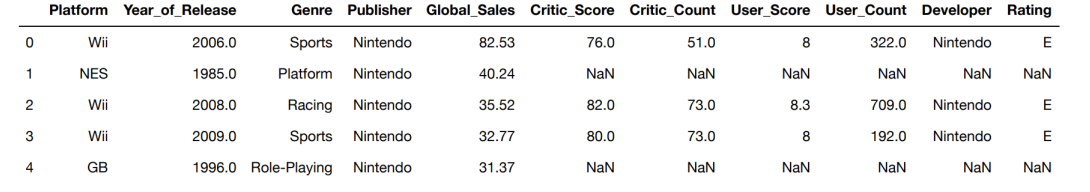
\includegraphics[scale=.6]{graphs/headdata.png}
        \caption{First 5 lines of data set after removing Sales Data apart from Global Sales}
        \label{fig:N20}
    \end{figure}
\end{frame}
    
\begin{frame}
    \frametitle{Cleansing the data}
    Steps:
    \begin{enumerate}
    \item Remove the rows containing missing data that cannot be imputed. (Platform, Genre, Publisher, Year of Release)
    
    \item Replace the missing values with the median of the column. (Critic Score, User Score, Critic Count, User Count)
    \item Replace categorical data with dummy variables (one-hot-encoding) (Genre, Publisher) and drop one column of each to decorrelate the columns. 
    
    \end{enumerate}
\end{frame}
\begin{frame}{Dropping categorical data}
    \begin{itemize}
        \item Dropping [Rating, Publisher, Japan Sales, EU Sales, Other Sales]
        
        \item On dropping rating: 
        \begin{figure}[H]
        \centering
        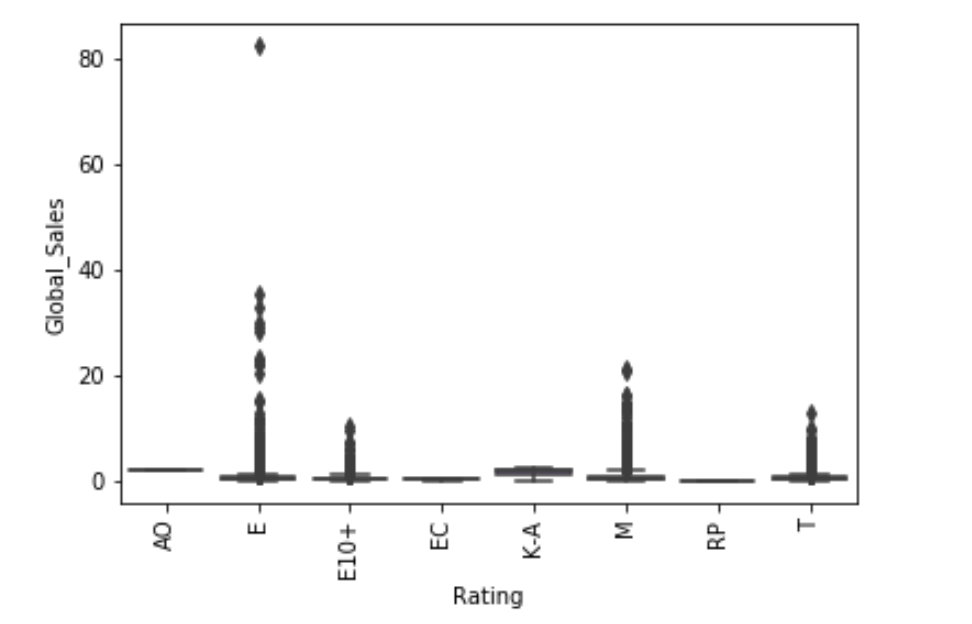
\includegraphics[scale=0.5]{graphs/rating.png}
        
    \end{figure}
    \item 
    Although there seems to exist a correlation, between rating and global sales. Our models worked better with its exclusion..so we dropped it!
    \end{itemize}
\end{frame}
\begin{frame}
    \frametitle{Preprocessing}
    

    \begin{itemize}
    \item In order to learn which features are important, I used a correlation matrix to plot the dependencies of variables on features like global sales.
       
    
     \end{itemize}   
    \begin{figure}[H]
        \centering
        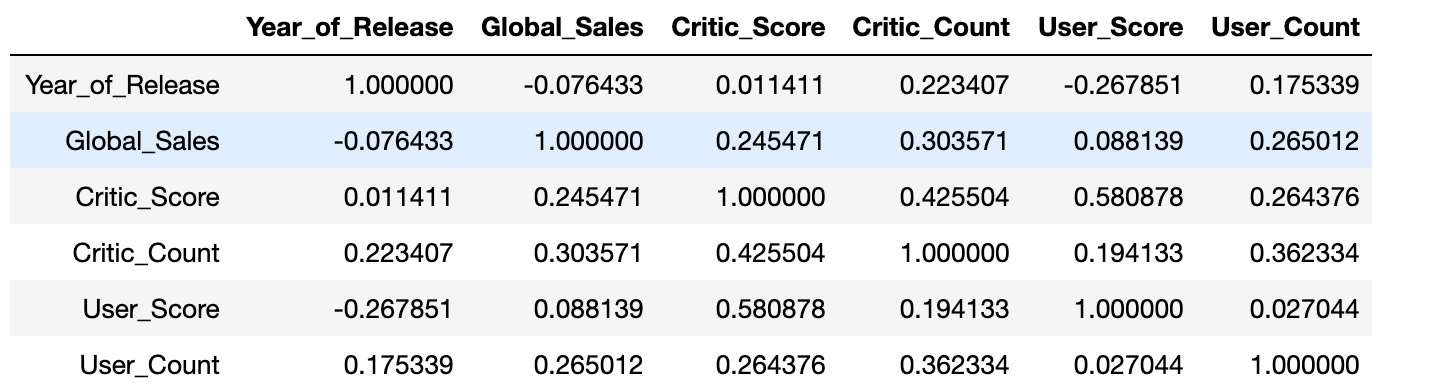
\includegraphics[scale=0.5]{graphs/correlationmat.png}
        \caption{Correlation Matrix}
        \label{fig:N20}
    \end{figure}
\end{frame}

\begin{frame}
    \frametitle{Preprocessing}
    \begin{itemize}
    \item I then plot the correlation matrix as a scatter plot to get a better idea of features to drop / include. 
    
     \begin{figure}[H]
        \centering
        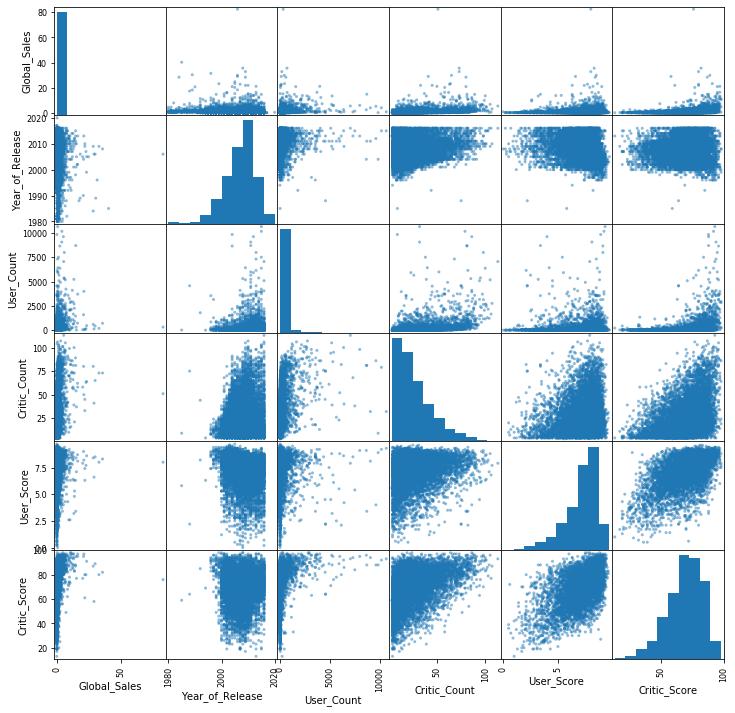
\includegraphics[scale=0.25]{graphs/plotcorr.png}
        \caption{Correlation Matrix Scatter Plot}
        \label{fig:N20}
    \end{figure}
    
    \end{itemize}
\end{frame}

\begin{frame}[fragile]
    \frametitle{Median Imputation, Failed KNN imputation}
    
    \begin{itemize}
    \item 
    We replaced the NaN values with the median of the column. (Critic Score, User Score, Critic Count, User Count). 
       \begin{lstlisting}[language=Python]
from sklearn.impute import SimpleImputer as Imputer
imp = Imputer(strategy="median")
attributes=["Critic_Score", "User_Score", "Critic_Count", "Critic_Count","User_Count"]
for item in attributes:
    game[item]=imp.fit_transform(game[[item]]).ravel()

      \end{lstlisting}
    \item Attempt to KNN, not ultimately used. 
    Using label encoder to first numerically label categorical data, then imputing using KNN. 
    \begin{lstlisting}[language=Python]
features_to_label=["Platform", "Genre","Publisher", "Rating", "Developer"]

for items in features_to_label:
    game.loc[~game[items].isnull(),[items]]=labelencoder.fit_transform(game.loc[~game[items].isnull(),[items]])
    #Changing all features to float64
    game["Developer"]= pd.to_numeric(game["Developer"])
game["Rating"]= pd.to_numeric(game["Rating"])
#KNN
knnimp=KNNImputer()
game=knnimp.fit_transform(game) 
      \end{lstlisting}


    \end{itemize}
\end{frame}


\begin{frame}[fragile]
    \frametitle{Median Imputation, Failed KNN imputation}
    \begin{itemize}
    \item Result of KNN Imputation was a success in regular linear regression where we saw a reduction in RMSE from 2.15 to 1.91 but did not as work well for the other models. So we did not implement this. 
    \n
    \begin{figure}[H]
        \centering
        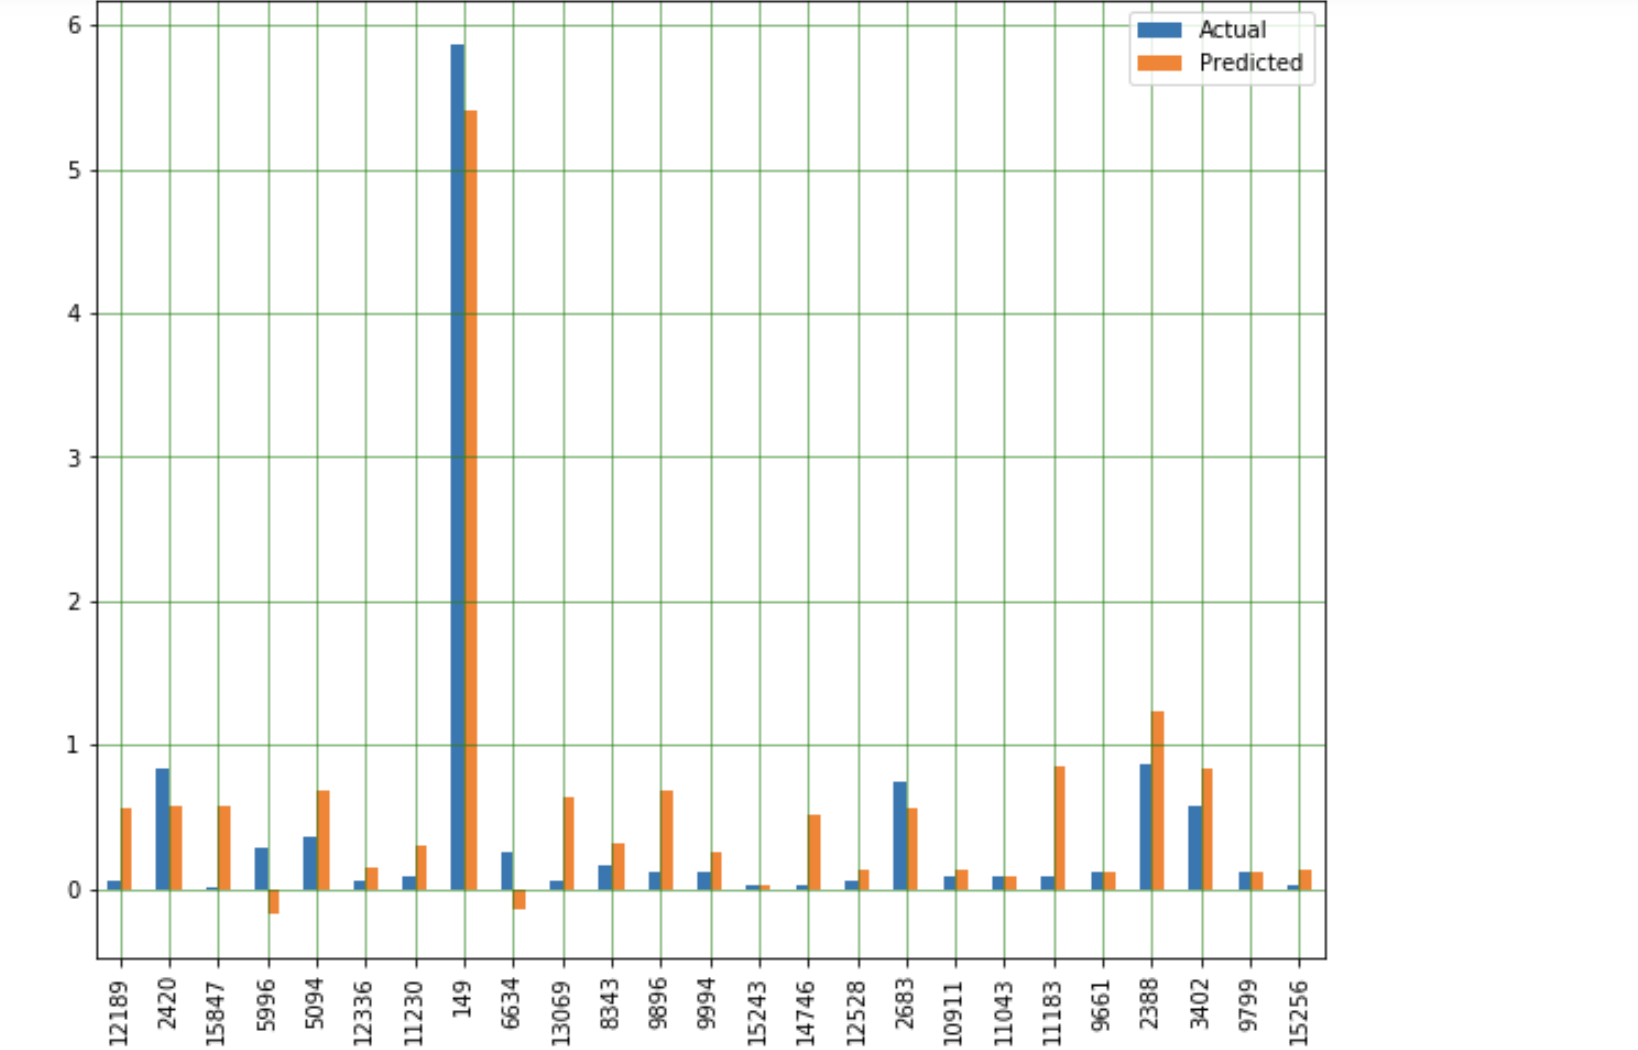
\includegraphics[scale=0.25]{graphs/improvement.png}
        \caption{Predicted to Actual Values}
        \label{fig:N20}
    \end{figure}
    \end{itemize}
\end{frame}


\begin{frame}[fragile]
    \frametitle{Using One hot-encoding}
    \begin{itemize}
        \item \underline {The why of using Onehot encoding and deletion of one column:} 
        
        \n 
        \n 
        Categorical data can not be used in any kind of models we wanted to implement. Lebel encoding was not sufficient. We decided to drop one column from each categorical data type because we would like to avoid non uniqueness and de-correlate the columns.  
        \item One-hot encoding, dropping 1st column 
    \begin{lstlisting}[language=Python]
    cat_features=["Rating", "Developer","Platform","Genre","Publisher"]

full_pipeline = ColumnTransformer([ # one hot encoding using this python pipeline function. very useful. Analogous to a design matrix
    ('cat', OneHotEncoder(handle_unknown='ignore'), cat_features)
])
X=full_pipeline.fit_transform(X)
    \end{lstlisting}
    \end{itemize}
\end{frame}